\subsection*{Ruteo}

Considere el siguiente código:

\lstinputlisting[style=mypy]{Code/AjedrezRuteo.py}


\newpage

Realice el ruteo del programa anterior e indique qué es lo que imprime. Cada vez que el valor de una variable cambie, escríbalo en una nueva fila de la tabla. Recuerde que si una variable es de tipo string, debe colocar su valor entre comillas simples ’ ’ o dobles " ".

\begin{figure}[H]
    \centering
    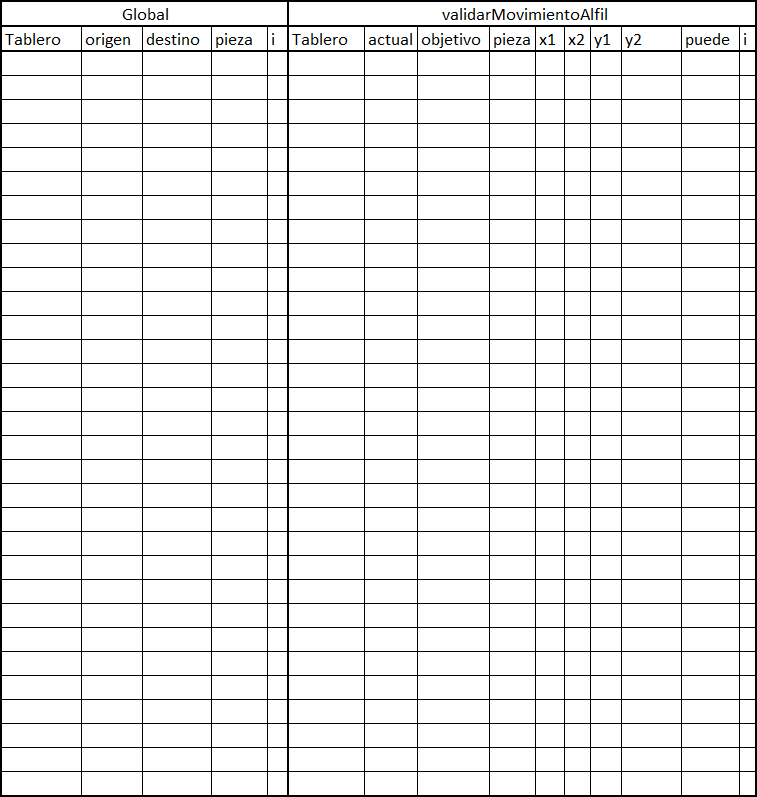
\includegraphics[width = 0.8 \textwidth]{Imagenes/tablaRuteo.png}
\end{figure}

\begin{figure}[H]
    \centering
    
\includegraphics[width = 0.4 \textwidth]{Imagenes/consola.png}
    \caption{Pantalla}
\end{figure}
